\documentclass[12pt,letterpaper]{article}

% Librerías a utilizar
\usepackage{float} % para libre imagen
\usepackage{listings}  %bloque de codigo 
\usepackage[utf8]{inputenc}	% Codificación 
\usepackage[spanish]{babel}	% Idioma
\usepackage{natbib}			% Bibliografía
\usepackage{graphicx}		% Imagenes
\usepackage{indentfirst}		% Sangría
\usepackage{amsmath, amsfonts, amssymb}	% Figuras matemáticas
\usepackage{url}    % URL
\renewcommand{\listtablename}{Índice de tablas}
\renewcommand{\tablename}{Tabla}

\usepackage[left=3cm,right=2cm,top=2cm,bottom=3cm]{geometry}

\setlength{\parindent}{2cm}	% Sangría en los párrafos
\renewcommand{\baselinestretch}{1.5}	% Interlineado

% Renombrar ciertos títulos del texto
\renewcommand\spanishcontentsname{Tabla de contenidos}
\renewcommand\spanishrefname{Bibliografía}

% Inicio del documento
\begin{document}

%%%%%%%%% PORTADA %%%%%%%%%

\newpage
\vspace*{-1cm}
% Logo institucional
\begin{picture}(18,4)(0,30)
	\put(-100,-20){
\includegraphics[scale=0.7]{./images/logo_usach.jpg}}
\end{picture}

\sloppy
\thispagestyle{empty}
\vspace*{2cm}

% Datos institucionales
\begin{center}
	{\bf \mbox{\large UNIVERSIDAD DE SANTIAGO DE CHILE}}\\
	{\bf \mbox{FACULTAD DE INGENIER\'IA}}\\
	{\bf \mbox{DEPARTAMENTO DE INGENIER\'IA INFORM\'ATICA}}\\
\end{center}

	\vspace{4cm}
	%Nombre asignatura
	\begin{center}
	\Large
		\textbf{Sistemas de comunicación}
	\end{center}
	
	%Título del trabajo
	\begin{center}
	\Large
		\textbf{Laboratorio N 1: Capa de enlace}
	\end{center}
	
	
	% Datos personales
	\vspace*{3.25cm}
	\begin{flushright}
		\begin{tabular}[t]{l l}
			Integrantes: &Nicolás Gutiérrez  \\			\\
			Ayudantes: &Catalina Morales\\
			           &Fernanda Muñoz\\\\
			
			Profesor(a): &Carlos Gonzalez Cortes

		\end{tabular}
	\end{flushright}
	\begin{center}
		\vspace{1.5cm}
		\today
	\end{center}

\newpage
\tableofcontents
\thispagestyle{empty}

\newpage
\renewcommand{\thepage}{\arabic{page}}
\setcounter{page}{1}

% Capítulos agregados 
\section{Introducción}

Durante las últimas décadas se ha visto una explosión en el uso de internet, según Europa Press (2018) \cite{ElTiempo} para el año 2018 el 51,2\% de la población mundial tenía acceso a internet. Internet forma parte del día a día en la mayoría de los hogares del mundo y, sin embargo, muchas personas desconocen cómo funciona realmente. Es por lo que en este informe se explorará las capas de los modelos y en específico la que corresponde a la capa de enlace o de enlace de datos (según el modelo que se esté estudiando).  \\

\noindent La capa de enlace es la encarga del intercambio de datos de cualquier computador o host y la red a la cual está conectado. Su principal objetivo es la de proveer una comunicación segura entre dos nodos pertenecientes a una misma red. Las principales funciones de la capa son: 

\begin{enumerate}
    \item Estructuración de mensajes en tramas
    \item Direccionamiento
    \item Control de errores
    \item Control de transición y flujo de datos
\end{enumerate}


\noindent ¿Cómo funciona la capa de enlace? ¿Qué relación tiene la capa de enlace con la capa física?  son algunas de las preguntas que se buscan responder con el presente documento. Además, en este informe se explorará el funcionamiento práctico de las capas física y de enlace haciendo un análisis de la red local, pasando por los dispositivos conectados a la red como por la velocidad de trasmisión que tienen estos.

\section{Marco Teorico}

\noindent En esta sección se busca explicar conceptos importantes que son utilizados durante el documento.

\subsection{Dirección MAC}

\noindent Cuando se habla de una dirección MAC se hace referencia de la dirección física de un dispositivo la cual es un identificador único que cada fabricante le asigna a la tarjeta de red de sus equipos. La dirección MAC está formadas por 48 bits representados generalmente por dígitos hexadecimales y tienen la forma: \verb|00:1e:c2:9e:28:6b|. Las direcciones MAC pueden ser utilizadas para permitir o denegar el acceso de determinados dispositivos a una red \cite{MAC}.


\subsection{Herramientas de Linux}

\noindent A continuación se describen las herramientas/programas utilizadas en el documento, estas herramientas o programadas de análisis son en su mayoría propias del sistema operativo Linux:

\begin{enumerate}
    \item \textbf{nmap} - Se utilizará para averiguar la topología de la red.
    \item \textbf{ifconfig} - Es la utilidad principal usada para configurar las interfaces de red.
    \item \textbf{Iperf3} - Es una utilidad para medir la velocidad de un enlace en internet.
    \item \textbf{Wireshark} - Es un analizador de protocolos que permite realizar capturas de tráfico de la red en tiempo real y obtener todos los datos de cada paquete involucrado.
\end{enumerate}


\subsection{Protocolo ARP}

\noindent El Address Resolution Protocol (protocolo de resolución de direcciones) es un protocolo de importancia en la transmisión de tramas por el internet debido a que ayuda a obtener las direcciones físicas de los dispositivos (lo que no puede hacer el protocolo de internet) además de almacenar en caché estas direcciones. Este protocolo envía una consulta a la dirección de difusión de la red y se espera que cada dispositivo responda a esa consulta. En síntesis, este protocolo permite que la dirección de internet sea independiente de la dirección de los dispositivos conectaos por LAN, disponibilizado la dirección física. 

\subsubsection{Tablas ARP}

\noindent ARP se encarga de la traducción de las direcciones IP a direcciones MAC por medio de tablas ARP. Sería una especie de base de datos donde se guarda la información de la ip y la MAC de un dispositivo. Para ser técnicos esta información es guardada en la caché y al estar en la caché se borran cada cierto tiempo. 

\begin{figure}[!h]
	\centering
	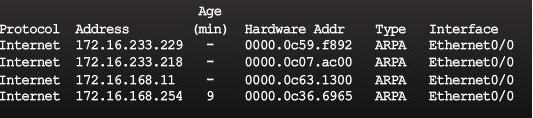
\includegraphics[scale=0.9]{images/arpexample.png}
	\caption{Imagen de ejemplo de una talba ARP}
	\label{arpexa}
\end{figure}

\noindent En general estas tablas poseen la información de la ip del dispositivo y la dirección física o MAC


\section{Desarrollo y resultados}

A continuación, se detalla todo el desarrollo de la experiencia exponiendo como se hizo cada parte del enunciado. Cabe destacar que el desarrollo fue realizado en un sistema operativo Linux en base Debian, en específico se utilizó \textbf{elementary OS}.

\subsection{Capa física y de enlace}
Primeramente, se ha realizado un análisis de la red local, pasando desde los dispositivos que están conectados a la red, hasta porque medios lo están, pero primero se debe conocer las características asociadas a la red y las del mismo dispositivo donde se están ejecutando las pruebas. Entonces con la herramienta \verb|ifconfig| se puede saber cuál es la ip local del dispositivo además de un rango de ip de la red:

\begin{figure}[!ht]
	\centering
	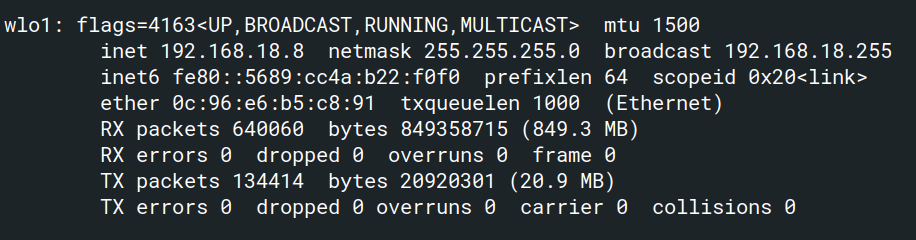
\includegraphics[scale=0.5]{images/ifconfig.png}
	\caption{Resultado de la ejecución de ifconfig}
	\label{if}
\end{figure}

\noindent Como se puede ver la figura \ref{if}, el dispositivo tiene la ip local \verb|192.168.18.8| además de que la red tiene un rango de ip de \verb|192.168.18.0| a \verb|192.168.18.255|.
\noindent Ahora para obtener información del adaptador de red del dispositivo se puede utilizar el siguiente comando:

\begin{lstlisting}
$ sudo lspci -nn | grep -i network
\end{lstlisting}

\begin{figure}[!ht]
	\centering
	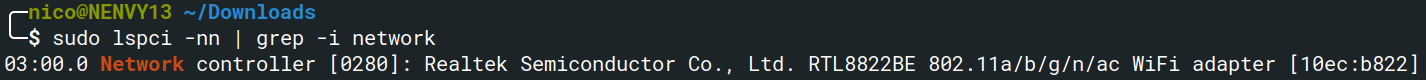
\includegraphics[scale=0.3]{images/lscpi.png}
	\caption{Resultado del comando lspci con información del adaptador de red}
	\label{lspci}
\end{figure}


\noindent Conociendo el dispositivo actual y el rango de ips local de la red se puede utilizar la herramienta \verb|nmap| para hacer un análisis de los dispositivos conectados a la red con sus ips y direcciones mac. Entonces si se ejecuta el siguiente comando: 

\begin{lstlisting}
$ sudo nmap -sn 192.168.18.1-255
\end{lstlisting}

\noindent Se obtiene la siguiente tabla de dispositivos:


\begin{table}[!h]
\begin{tabular}{|l|l|l|l|}
\hline
\textbf{Nombre de dispositivo} & \textbf{Capa física}  & \textbf{Dirección MAC} & \textbf{Dirección IP} \\ \hline
\_gateway(router)                 & \begin{tabular}[c]{@{}l@{}}Ethernet (802.3a) \\ WiFi 802.11a/b/g/n/ac\end{tabular}           & 24:a5:2c:4d:b4:17      & 192.168.18.1          \\ \hline
PC-Escritorio                  & Ethernet (802.3a)             & f0:79:59:92:b6:77      & 192.168.18.5          \\ \hline
Google-Home-Mini               & WiFi 802.11b/g/n/ac   & b0:2a:43:2d:86:84      & 192.168.18.6          \\ \hline
Desconocido                    & Wifi 802.11ac           & cc:9f:7a:3d:71:4c      & 192.168.18.7          \\ \hline
NENVY13                        & WiFi 802.11a/b/g/n/ac & 0c:96:e6:b5:c8:91      & 192.168.18.8          \\ \hline
HUAWEI\_Mate\_20\_l            & WiFi 802.11b/g/n/ac           & 88:bf:e4:21:12:b0      & 192.168.18.11         \\ \hline
Mi9T-MiTel?fono                & WiFi 802.11a/b/g/n/ac & a8:9c:ed:67:09:79      & 192.168.18.18         \\ \hline
Nintendo 3DS                   & WiFi 802.11b/g/n/ac   & 7c:bb:8a:64:b2:3b      & 192.168.18.19         \\ \hline
LG-TV-living                   & Ethernet (802.3a)             & c8:08:e9:be:6c:a4      & 192.168.18.21         \\ \hline

\end{tabular}
\caption{Tabla de resumen de dispositivos en la red local}
\end{table}

\noindent De lo anterior se puede elaborar un diagrama de red: 

\begin{figure}[H]
	\centering
	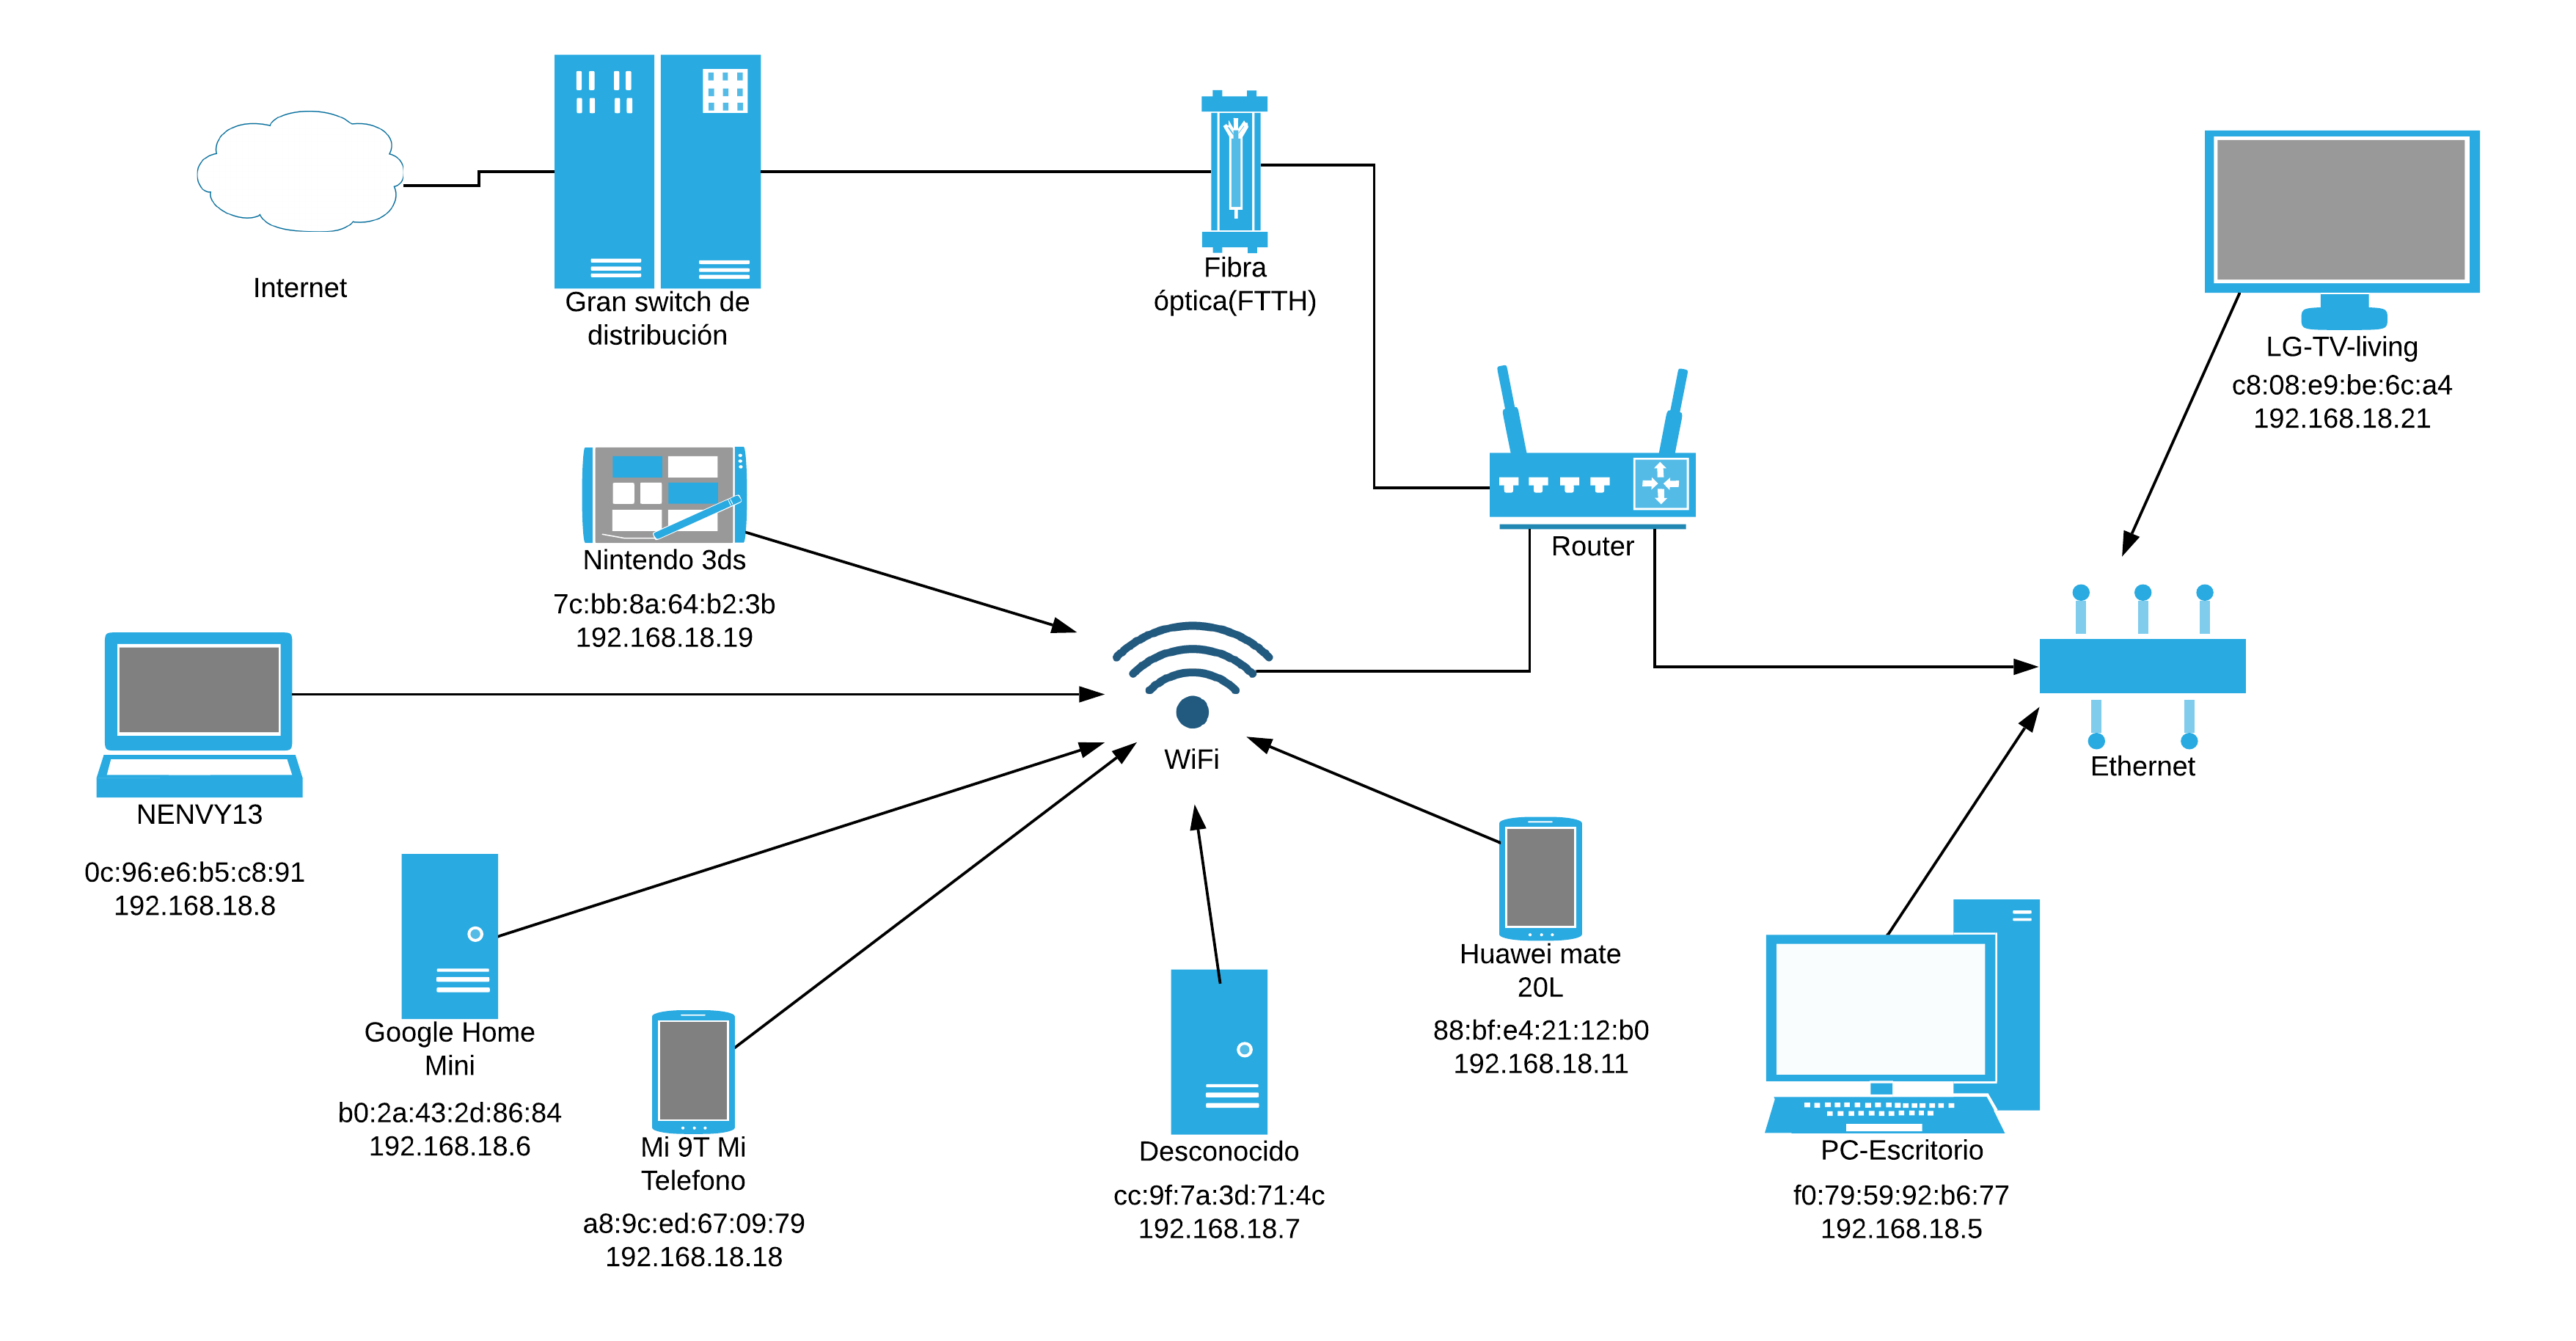
\includegraphics[scale=0.57]{images/Diagrama de Red (1).png}
	\caption{Diagrama de red con los dispositivos conectados al momento de hacer el análisis }
	\label{diag:red}
\end{figure}


\noindent Conociendo la red y las ips de los dispositivos se procede a hacer un análisis de la velocidad de transmisión entre dos dispositivos. Con ayuda de la herramienta \verb|iperf3| se ha creado un servidor en el dispositivo \textbf{PC-Escritorio} con la ip local \verb|192.168.18.5| . Cabe destacar que este dispositivo posee un sistema operativo Windows 10 el cual posee un subsistema de Linux en el cual se puede instalar \verb|iperf3|. Teniendo esto en cuenta en el dispositivo \textbf{PC-Escritorio} se establece el comando :

\begin{lstlisting}
$ iperf3 -s
\end{lstlisting}

\noindent Ahora en el dispositivo \textbf{NENVY13} con la ip local \verb|192.168.18.8| el cual está conectado al Wifi con 5G, se ejecuta el siguiente comando:

\begin{lstlisting}
$ iperf3 -c 192.168.18.5 -u -b XM
\end{lstlisting}



\noindent Donde X toma valores entre 1 a 1000, los cuales representan el ancho de banda en Megabits. Para esta sección se han hecho diferentes pruebas, modificando X, los cuales tomaron valores [1,10,100,200,300,400,500,1000] de lo que se obtuvo el siguiente gráfico:

\begin{figure}[!h]
	\centering
	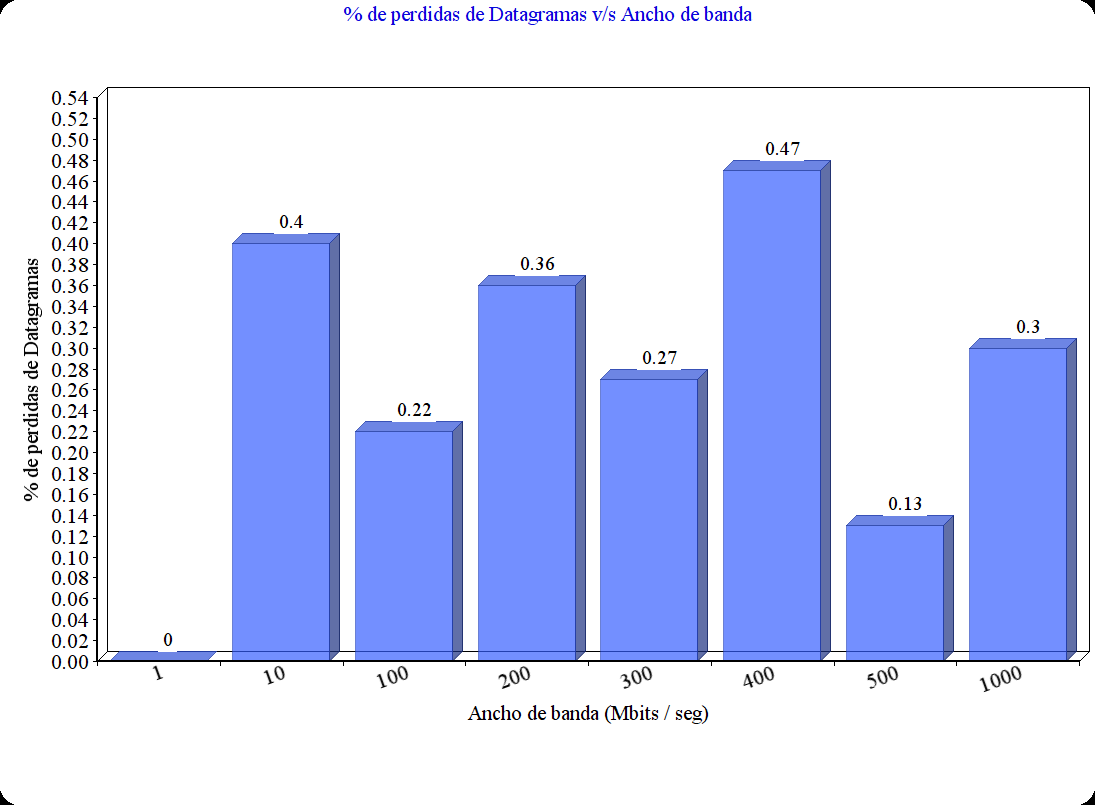
\includegraphics[scale=0.5]{images/graph.png}
	\caption{Gráfico del \% de datagramas perdidos v/s Ancho de banda en 5G}
	\label{diag:iperf3}
\end{figure}



\subsection{Protocolo ARP}
 
 \noindent En esta sección se estudiará el protocolo ARP mediante \verb|Wireshark|. En el Marco Teórico se puede encontrar más información sobre Wireshark y el protocolo ARP. 
 
 
 \subsubsection{Capturando paquetes con Wireshark}
 
 Primeramente, para empezar a capturar datos con Wireshark, se ha instalado la herramienta con el siguiente comando: 
 
 \begin{lstlisting}
$ sudo apt install libcap2-bin wireshark
\end{lstlisting}

\noindent Luego para comenzar a capturar paquetes con esta herramienta se utiliza el siguiente comando: 
 \begin{lstlisting}
$ sudo wireshark 
\end{lstlisting}

Al iniciar se debe colocar la interfaz de red que se está utilizando, en el caso particular de esta experiencia es \verb|wlo1|.

\noindent Es importante iniciarlo en modo súper usuario debido a que Wireshark necesita permisos para capturar todos los paquetes de la red. Luego, cuando ya se ha iniciado el programa,se comienza de inmediato la captura de paquetes que circulan por la red a los diferentes dispositivos.

\begin{figure}[!ht]
	\centering
	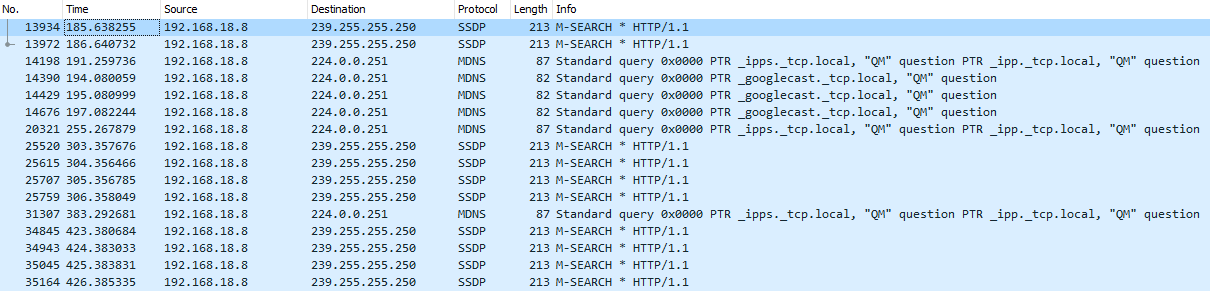
\includegraphics[scale=0.5]{images/wireshark1.png}
	\caption{Imagen de Wireshark capturando datos de los dispositivos conectados}
	\label{fig:wire1}
\end{figure}


\noindent Como se puede ver en la figura \ref{fig:wire1} Wireshark proporciona información sobre el origen y destino de la data que está circulando, aparte del protocolo utilizado. Lo interesante de esta aplicación es que se puede filtrar por ips y saber con qué ip se está comunicando cierto dispositivo. Por ejemplo, si se fija la ip de destino del \textbf{PC-Escritorio} (\verb|192.168.18.5|). Para fijar un filtro, en la parte superior de la tabla de datos, se puede colocar \verb|ip.dst == 192.168.18.5| lo cual da: 

\begin{figure}[!ht]
	\centering
	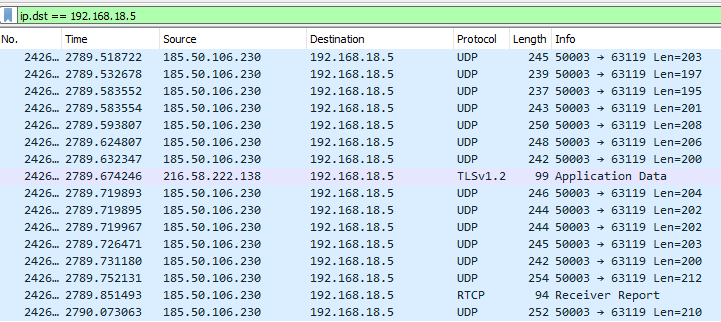
\includegraphics[scale=0.6]{images/wireshark2.png}
	\caption{Imagen de Wireshark con filtro de ip de destino}
	\label{fig:wire2}
\end{figure}


\subsubsection{Obteniendo información de las tablas ARP}

\noindent Como se veia en el capítulo de marco teórico, el protocolo ARP posee tablas almacenadas en caché que guardan datos de las direcciones físicas de los dispositivos de la red asociadas a una ip local. Es por eso que ahora se estudiará que datos se almacenan en el dispositivo de prueba \textbf{NENVY13} (\verb|192.168.18.8|).
\newline

\noindent Entonces antes de comenzar a obtener la tabla ARP actual, se partirá desde un comienzo con la tabla vacía. Para vaciar la tabla se ha utilizado el siguiente comando: 

 \begin{lstlisting}
$ sudo ip -s -s neigh flush all
\end{lstlisting}

\noindent Como ya se ha vaciado la tabla ARP del dispositivo, se puede obtener la tabla actual con el comando:

 \begin{lstlisting}
$ arp -n
\end{lstlisting}
 
 \noindent En el comando anterior, no existe mayor diferencia si se ejecuta en modo súper usuario o no. Entonces al ejecutar el código anterior se obtiene:
 
 \begin{figure}[!ht]
	\centering
	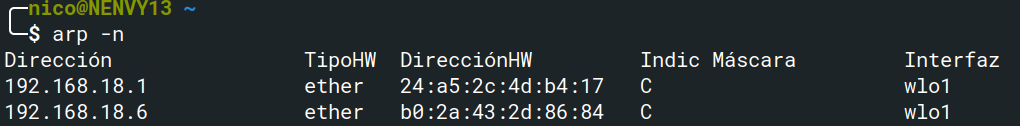
\includegraphics[scale=0.4]{images/arp_1.png}
	\caption{Imagen resultado de la tabla ARP luego de vaciarla}
	\label{fig:arp1}
\end{figure}
 
 \noindent Ahora para probar si la tabla se actualiza correctamente, se ha hecho \verb|$ ping 192.168.18.8| de los siguientes dispositivos:
 
 \begin{enumerate}
     \item PC-Escritorio (\verb|192.168.18.5|)
     \item Mi9T-MiTelefono (\verb|192.168.18.18|)
 \end{enumerate}
 
 \noindent Ahora se ha vuelto a ver la tabla ARP del dispositivo con el comando antes mencionado:
 
 \newpage
 
\begin{figure}[!ht]
	\centering
	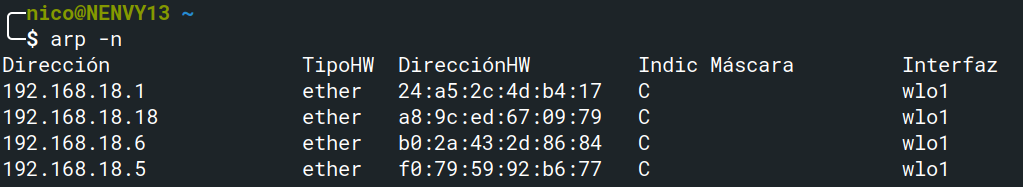
\includegraphics[scale=0.4]{images/arp_2.png}
	\caption{Imagen de la nueva tabla ARP después de hacer pings}
	\label{fig:arp2}
\end{figure}

\noindent Lo que continua en la siguiente sección se analizará que ocurre en Wireshark mientras se hace el ping al dispositivo.

\section{Análisis de Resultados}

En esta sección se dará respuesta y explicación de los resultados de la sección pasada. Es importante decir que se harán referencia a las Figuras mostradas en la sección anterior, por lo que se hará necesario volver a revisarlas en cierto punto. 

\subsection{Capa física y de enlace : Análisis de la red}

\noindent En la sección pasada se vio como se utilizaba la
herramienta \verb|iperf3| y \verb|nmap| para escanear la red en busca de sus dispositivos. De este escaneo, se obtuvo la tabla/cuadro \ref{if} con los 9 dispositivos conectados a la red. Pero de esto surge la siguiente duda ¿Cuantos dispositivos pueden estar conectados a la red ?, Una respuesta rápida seria tantos como la cantidad de ips pueda dar el router. \cite{maxMAC}. Entonces en el caso particular la cantidad maxima de dispositivos que puede aceptar el router son 253 (del 1 al 255, menos un que es utilizado por el propio router). Sin embargo, no es recomendable tener tantos dispositivos conectados debido al tráfico que generaría, ralentizando la velocidad de transferencia.
\newline

\noindent Ahora si se fija en la figura \ref{diag:red} que muestra el diagrama de red, se puede ver que un detalle de los dispositivos conectados tanto por Wifi y por Ethernet, cabe destacar que como el router trabaja con dual band en la señal wifi(2.4GHz y 5GHz), algunos dispositivos terminan conectándose a la señal por un protocolo distinto, por ejemplo, los dispositivos que se conectan al 5G utilizan 802.11a mientras que los que se conectan al 2.4G utilizan 802.11b/g/n/ac. También en este diagrama tiene un foco en la distribución interna de los dispositivos, ahora si se quiere saber más sobre lo que ocurre fuera del hogar, se puede investigar desde la página del proveedor de internet. En este caso sería \textbf{Mundo pacifico}.


\begin{figure}[!h]
	\centering
	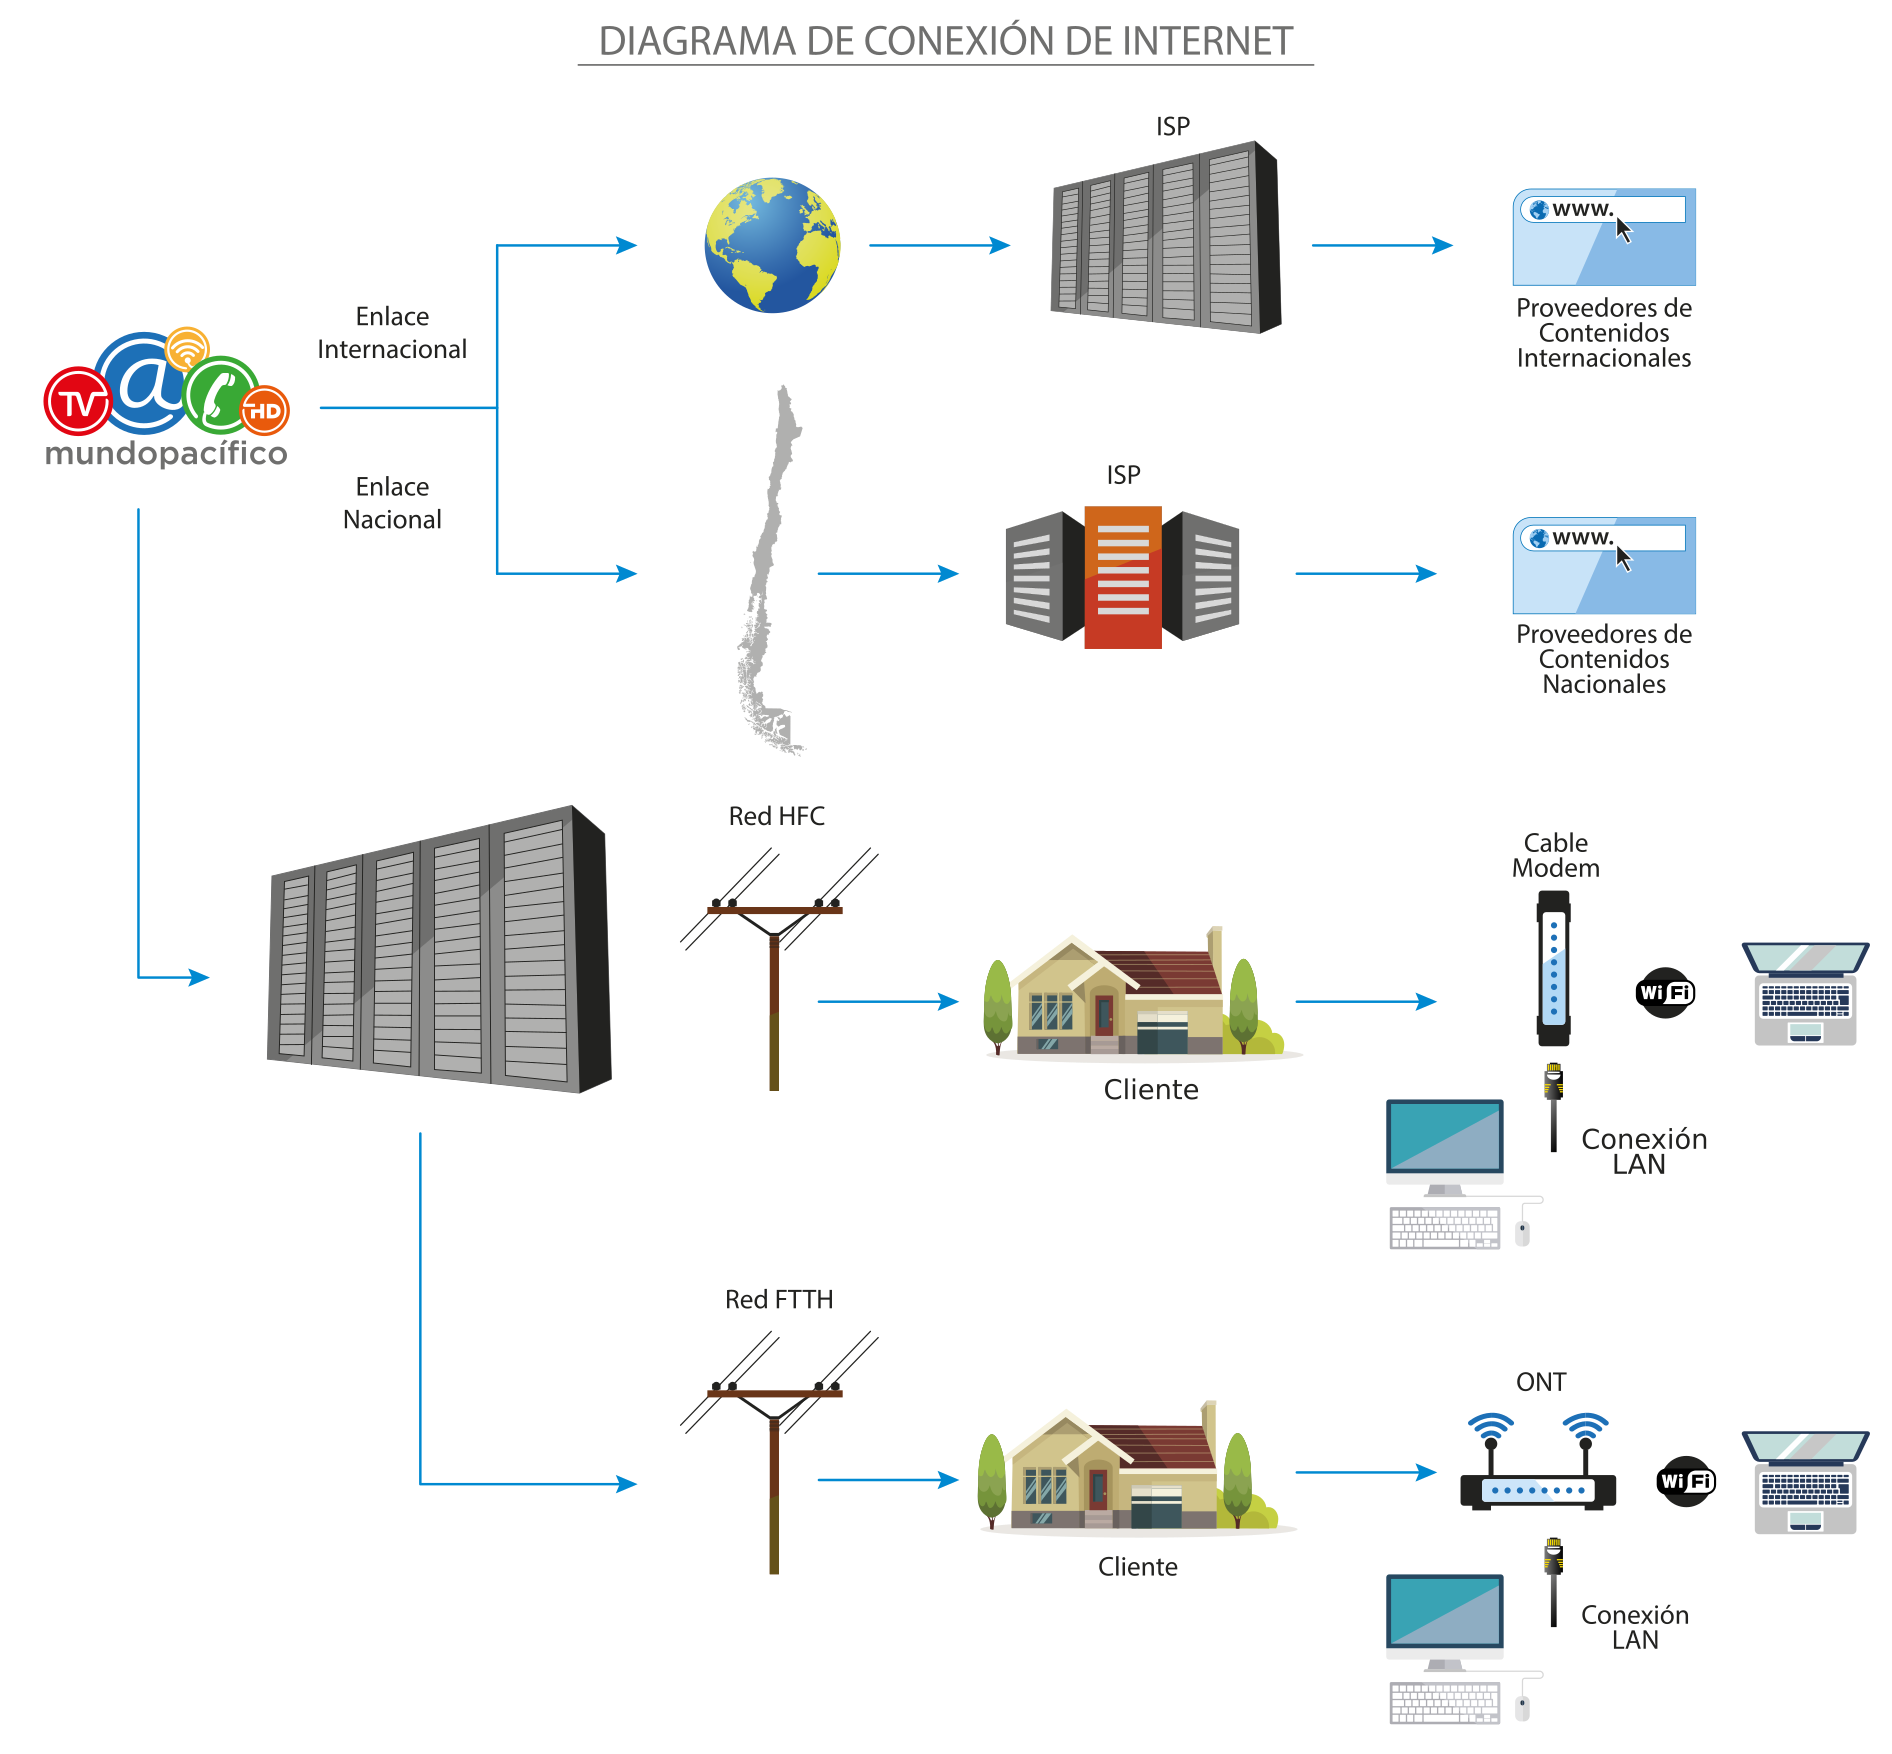
\includegraphics[scale=0.9]{images/diagrama-conexxion-net.png}
	\caption{Diagrama de conexión a internet fuera del hogar obtenido de Mundo Pacifico \cite{Mundo} }
	\label{diag:iperf3}
\end{figure}

\noindent Como se vio en la sección anterior, se ha realizado un test de velocidad entre los dispositivos \textbf{PC-Escritorio} (\verb|192.168.18.5|) que actúa como server y \textbf{NENVY13} (\verb|192.168.18.8|), el cual es donde se envían los paquetes. El resultado de dicho test se encuentra en el gráfico de la figura \ref{diag:iperf3} el cual si se analiza se puede ver que a primera vista no existe alguna relación con la tasa de pérdidas y el ancho de banda, además es importante mencionar el dispositivo NENVY13 se encontraba conectado al 5G del router, alcanzando una velocidad máxima de 425 Mbits/s entonces en la prueba de ancho de banda de 500 y 1000 no hubo diferencia de velocidad. Luego de esto surge la pregunta ¿Existirá alguna diferencia de la tasa de perdidas con el tipo de protocolo usando en la conexión? Para esto se ha repetido la experiencia, pero se ha conectado el dispositivo NENVY13 a la red 2.4G. Como resultado ha dado lo siguiente: 

\newpage

\begin{figure}[!h]
	\centering
	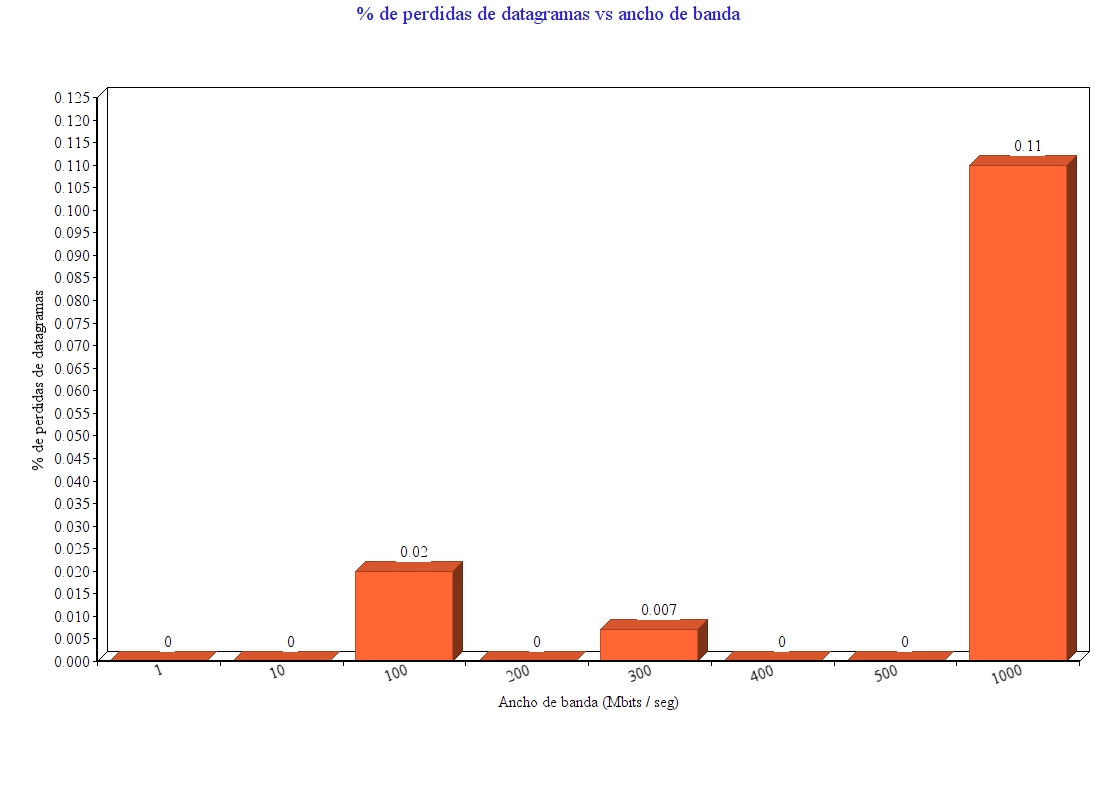
\includegraphics[scale=0.5]{images/barplots.png}
	\caption{Gráfico del \% de datagramas perdidos v/s Ancho de banda en 2.4G}
	\label{diag:iperf3}
\end{figure}

\noindent Como se puede ver la cantidad de Datagramas perdidos ha descendido de forma considerable, teniendo solo un máximo de 0.11\%, cabe destacar que la velocidad máxima alcanzada fue de 110 Mbits/s. Lo anterior puede significar que el 5G es mucho más inestable en cuanto a la transmisión que el 2.4G, sin embargo, su velocidad es mucha mayor a la del 2.4G.

\newline

\noindent Respecto a los datagramas, estos se pierden debido a las colisiones que existen dentro de la red, por ejemplo, si estuvieran solo estos 2 equipos en la red, habría una menor probabilidad de tener perdidas de datagramas. 

\subsection{Protocolo ARP}

Como se vio en el capítulo anterior, al momento de hacer de estar revisando las tablas ARP y vaciarlas, se puede ver en la figura \ref{fig:arp1} que la tabla si contiene algunas ips ¿Esto por qué se da?, primeramente si se ven las ips en la tabla se puede diferenciar la primera (\verb|192.168.18.1|), si se recuerda, esta ip corresponde a la ip del router por lo que es necesario que exista en la tabla ARP ya que el router siempre se está comunicando con el dispositivo.  Ahora la segunda ip (\verb|192.168.18.6|) corresponde a la ip del dispositivo de Google home mini. A primera vista, no se puede establecer una explicación de por qué se encuentra en la tabla ARP. Investigando un poco, este dispositivo escanea constantemente la red en busca de otros dispositivos compatibles con la integración de Google, entonces este dispositivo posee la información de cada equipo conectado a la red en su tabla ARP. 
\newline

\noindent Después de esta explicación, al momento de hacer ping a un dispositivo, el protocolo hace necesario guardar en la tabla ARP la información del dispositivo que está haciendo ping. Entonces cualquier dispositivo que haga ping a otro dentro de la red, este último sabrá quién le está mandando información ya que lo tendrá agregado a su propia tabla, lo cual explica la figura \ref{fig:arp2}. 


\noindent Ahora bien, una cosa es saber que ocurre dentro de cada dispositivo pero ¿Que ocurre en la red cuando se envía un ping a un dispositivo? Para responder esta pregunta, es necesario utilizar Wireshark, y colocar el siguiente filtro \verb|ip.dst==192.168.18.8|, lo cual fija la ip de destino del dispositivo NENVY13. 


\begin{figure}[!h]
	\centering
	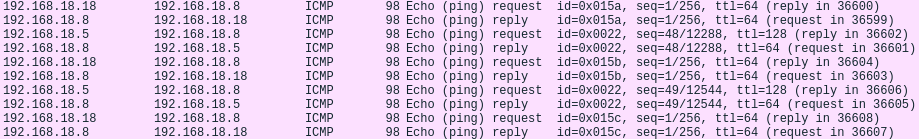
\includegraphics[scale=0.5]{images/wire3.png}
	\caption{Imagen de lo que ocurre en Wireshark mientras se realizan los ping al equipo NENVY13}
	\label{diag:iperf3}
\end{figure}

\noindent Como se puede ver para la comunicación se utiliza el protocolo ICMP, el cual es sirve para mandar mensajes entre dos dispositivos con información sobre el estado de la red y devolver mensajes sobre problemas con datagramas al remitente del paquete \cite{icmp}. En este caso lo que se envía es una información de control y por el comando: \verb|echo (ping)|. 

\noindent Si se ve en la info , se puede notar que cada paquete de ping es acompañado de un \textit{Request} o \textit{Reply} dependiendo en qué dirección vaya. Si el destino es \verb|echo (ping)| será una \textit{Request} caso contrario, si el inicio es \verb|echo (ping)| será una \textit{Reply} .
\newline

\noindent Se se analiza el tráfico general de la red se puede ver que este es normal y se puede notar que la mayor cantidad de paquetes son enviados desde el dispositivo \textbf{Google home mini} ya sea a los dispositivos conectados como a los servidores de Google, en específico se hacen a la ip \verb|172.217.192.97| la cual con cualquier \textit{Whois} en internet se puede saber a quién pertenece.

\section{Conclusiones}
En esta experiencia se logró implementar lo solicitado, es decir, se pudo realizar un análisis de la capa física y la de enlace, pasando desde un análisis de la estructura de toda la red hasta un análisis del tráfico de la misma red.
\newline

\noindent Como se pudo ver en la sección de análisis la tasa de pérdidas de datagramas varia si se utiliza un Wifi 2.4G o un 5G. Esto se debe a que, a mayor tasa de envío de bits, mayor será las colisiones que se generarán dentro de la red, provocando perdidas de datagramas. Otro de los puntos de los puntos de este análisis, se pudo dar cuenta de dispositivos que estaban conectados a la red y no se tenía alguna idea de que dispositivo podría ser. Este es el caso del dispositivo desconocido con ip \verb|192.168.18.7| el cual se detectó con el análisis de red y se terminó bloqueando desde el router.
\newline

\noindent Respecto al análisis de paquetes se pudo dar cuenta de la gran cantidad de protocolos utilizados en la comunicación de dos dispositivos en la red, aparte de la gran importancia del protocolo ARP en el nivel de enlace. La herramienta Wireshark utilizada resultó ser una herramienta poderosa en la captura de paquetes de información, sin embargo, resulta ser de doble filo ya que también es posible utilizarla para acceder a información delicada dentro de una red pública (cafés, cines, etc)
\newline

\noindent La existen de un gran tráfico en la red solo da cuenta de la gran importancia de la comunicación por esta gran con sus variados protocolos llamada internet, con el gran desarrollo del IoT(internet de las cosas) cada vez estará aumentando los di positivos en los hogares por lo que futuramente se necesitará  de mejores arquitecturas de redes y dispositivos de enrutamiento capaces de soportarlo.


\clearpage


\begin{thebibliography}{X}
\bibitem{ElTiempo} Europa Press. (2018, Diciembre 13). <<Más de la mitad de la población mundial tiene acceso a internet>>. Visitado en Mayo 29, 2020, desde https://www.eltiempo.com/tecnosfera/novedades-tecnologia/mas-de-la-mitad-de-la-poblacion-mundial-tiene-acceso-a-internet-304778


\bibitem{maxMAC} Jiménez, J. (2019, Marzo 24). <<Este es el máximo número de dispositivos que pueden conectarse a un router y así puedes modificarlo. >> Visitado en Junio 01, 2020, desde https://www.redeszone.net/2019/03/24/numero-maximo-dispositivos-router/

\bibitem{Mundo} Mundo Pacifico (2020, Mayo 13). <<Características De Servicio De Internet.>> Visitado en Junio 01, 2020, desde https://www.mundopacifico.cl/terminos-regulaciones/caracteristicas-de-servicio-de-internet/

\bibitem{icmp} How, K. (2019, Marzo 5). <<¿Qué es el protocolo ICMP y cómo funciona?>> Visitado en Junio 03, 2020, desde https://www.ionos.es/digitalguide/servidores/know-how/que-es-el-protocolo-icmp-y-como-funciona/

\bibitem{MAC} FM, Y. (2017, Octubre 5). Qué es la dirección MAC de tu ordenador, del móvil o de cualquier dispositivo. Visitado en Junio 3, 2020, desde https://www.xataka.com/basics/que-es-la-direccion-mac-de-tu-ordenador-del-movil-o-de-cualquier-dispositivo

\end{thebibliography}



\nocite{*}

\end{document}